\documentclass[t]{beamer}
\usetheme[deutsch]{KIT}
\setbeamercovered{transparent}
\setbeamertemplate{navigation symbols}{}
\graphicspath{ {Systemmodelle/images_blank/} }

\KITfoot{ Croggle - Praxis der Softwareentwicklung WS 13/14}
\usepackage[utf8]{inputenc}
\usepackage{ngerman}
\usenavigationsymbols

\title{Croggle}
\subtitle{PSE - Planungsphase \\[0.3cm]
Lukas Böhm $\cdot$ Tobias Hornberger $\cdot$ Jonas Mehlhaus \\ Iris Mehrbrodt  $\cdot$ Vincent Schüßler $\cdot$ Lena Winter}

\institute[IPD]{Institut für Programmstruktutren und Datenorganisation}

\TitleImage[height=\titleimageht]{title-image-darkgray.png}

\AtBeginSection[]
{
  \begin{frame}
    	\frametitle{Übersicht}
    	\tableofcontents[currentsection]
  \end{frame}
}

\begin{document}

\begin{frame}
        \maketitle
\end{frame}

\begin{frame}
        \frametitle{Übersicht}
        \addcontentsline{toc}{section}{}
        \tableofcontents
\end{frame}

\section{Zielsetzung}
\begin{frame}
	Entwickeln einer Lernapplikation für Kinder:\\
	\begin{itemize}
		\item Zielgruppengerechte Bedienung \pause
		\item Anhaltende Motivation \pause
		\item Kontrolle des Lernfortschritts
	\end{itemize}
\end{frame}

\section{Umsetzung}
\begin{frame}
	\frametitle{Bedienung}
	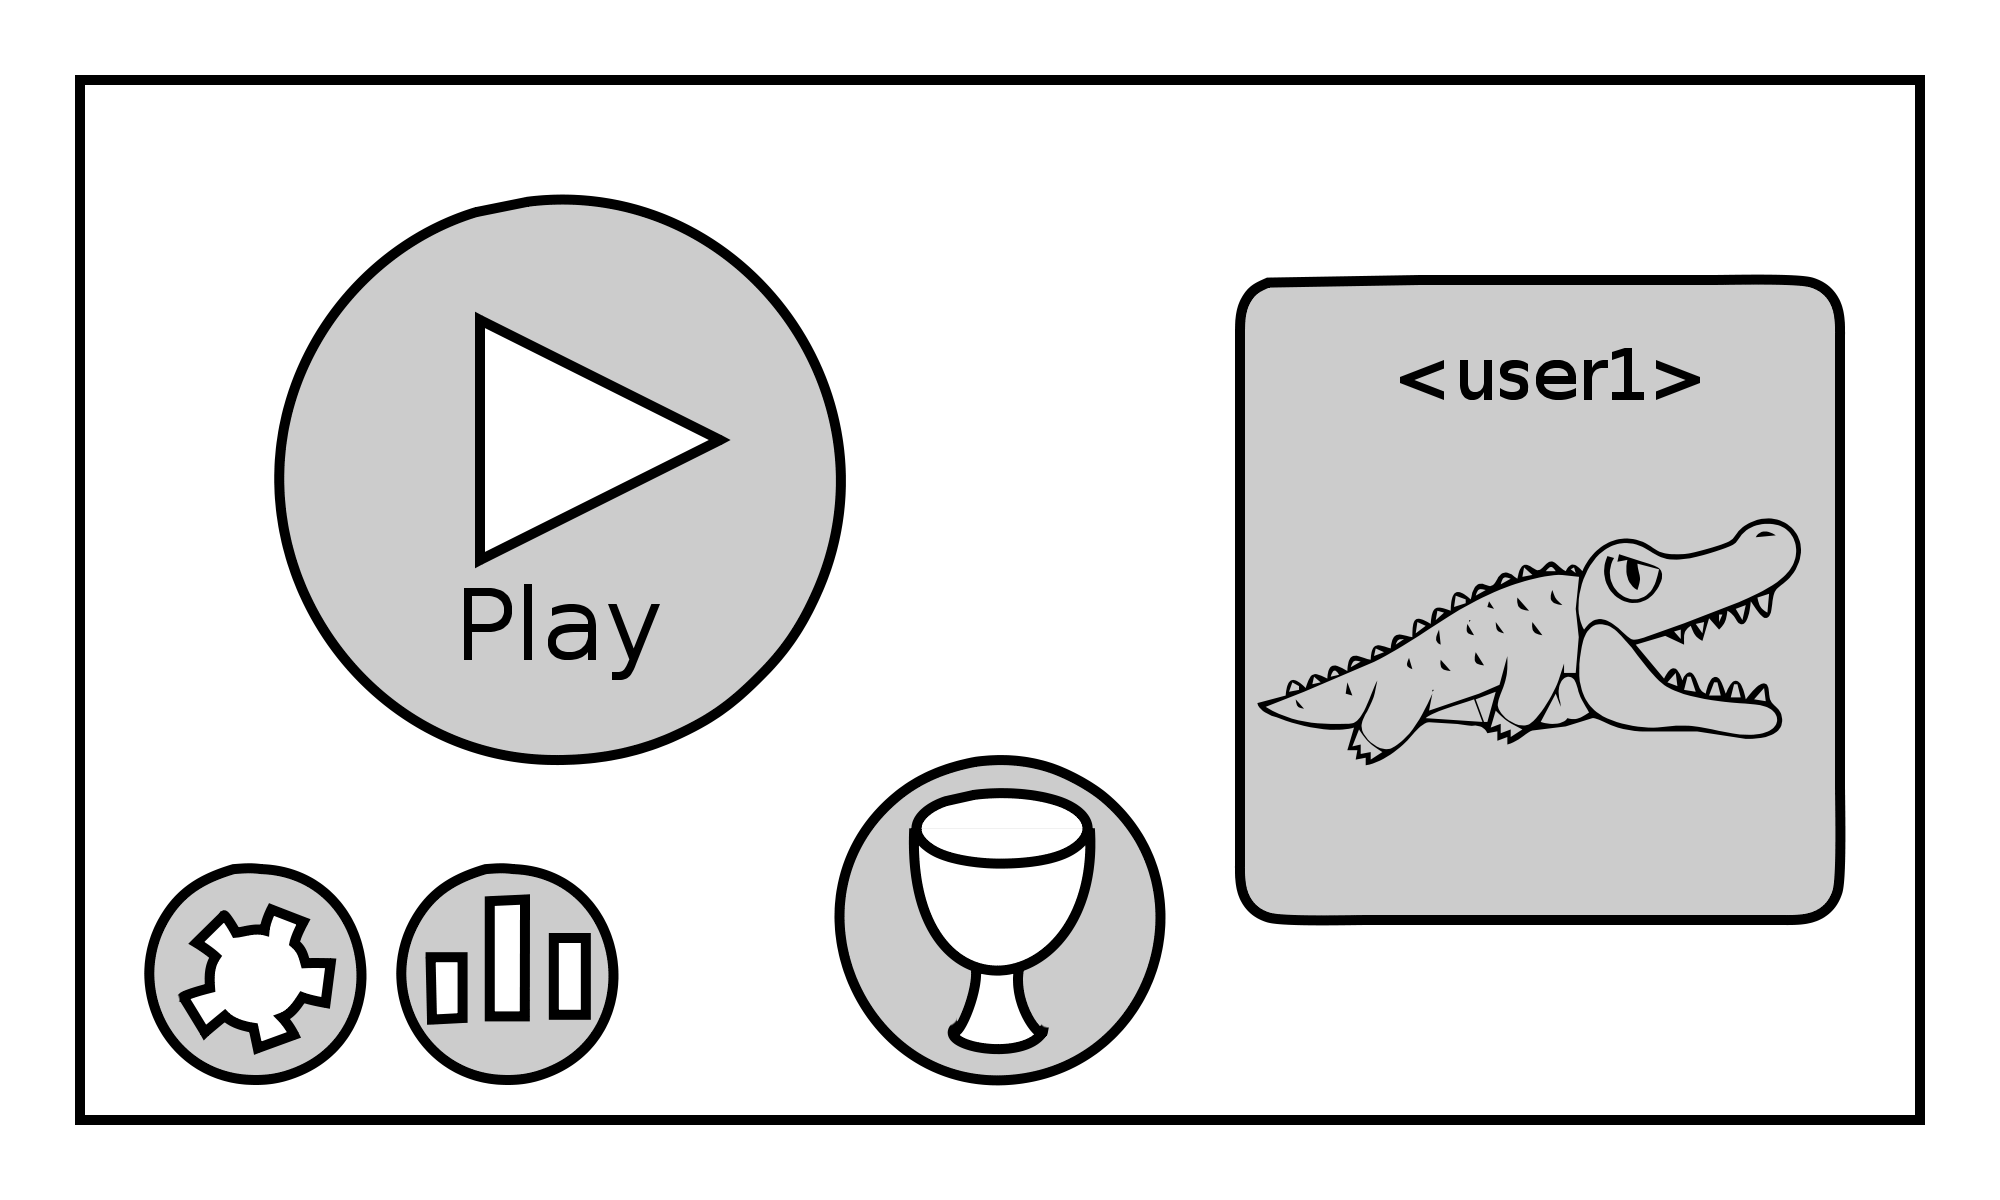
\includegraphics[height=\textheight]{main_menu.png}
\end{frame}
\begin{frame}
	\frametitle{Bedienung}
	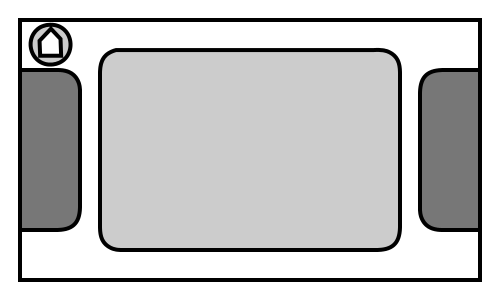
\includegraphics[height=\textheight]{level_overview.png}
\end{frame}
\begin{frame}
	\frametitle{Bedienung}
	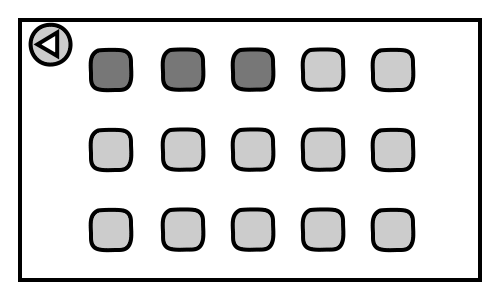
\includegraphics[height=\textheight]{level_overview_detail.png}
\end{frame}
\begin{frame}
	\frametitle{Bedienung}
	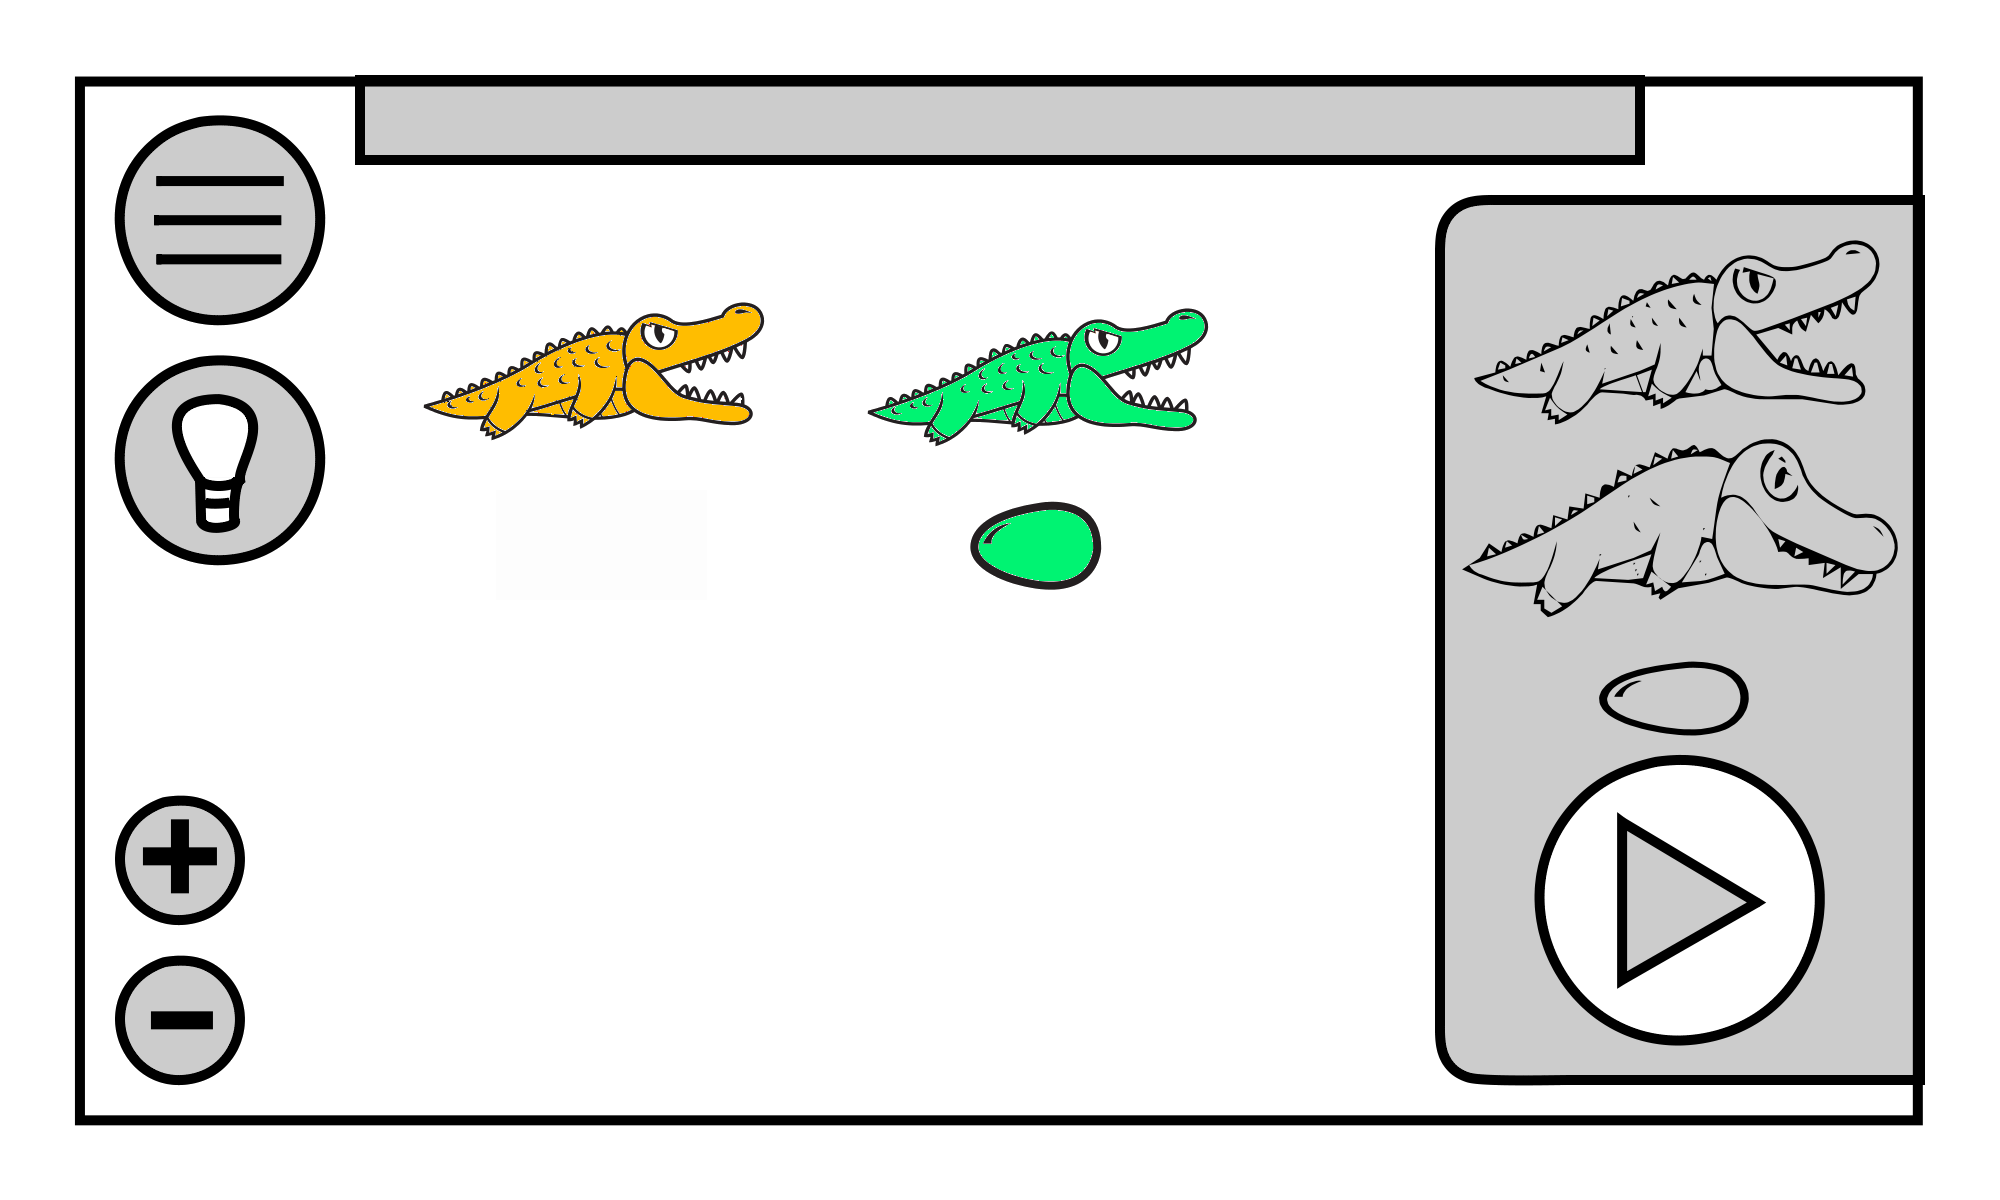
\includegraphics[height=\textheight]{level_start.png}
\end{frame}
\begin{frame}
	\frametitle{Bedienung}
	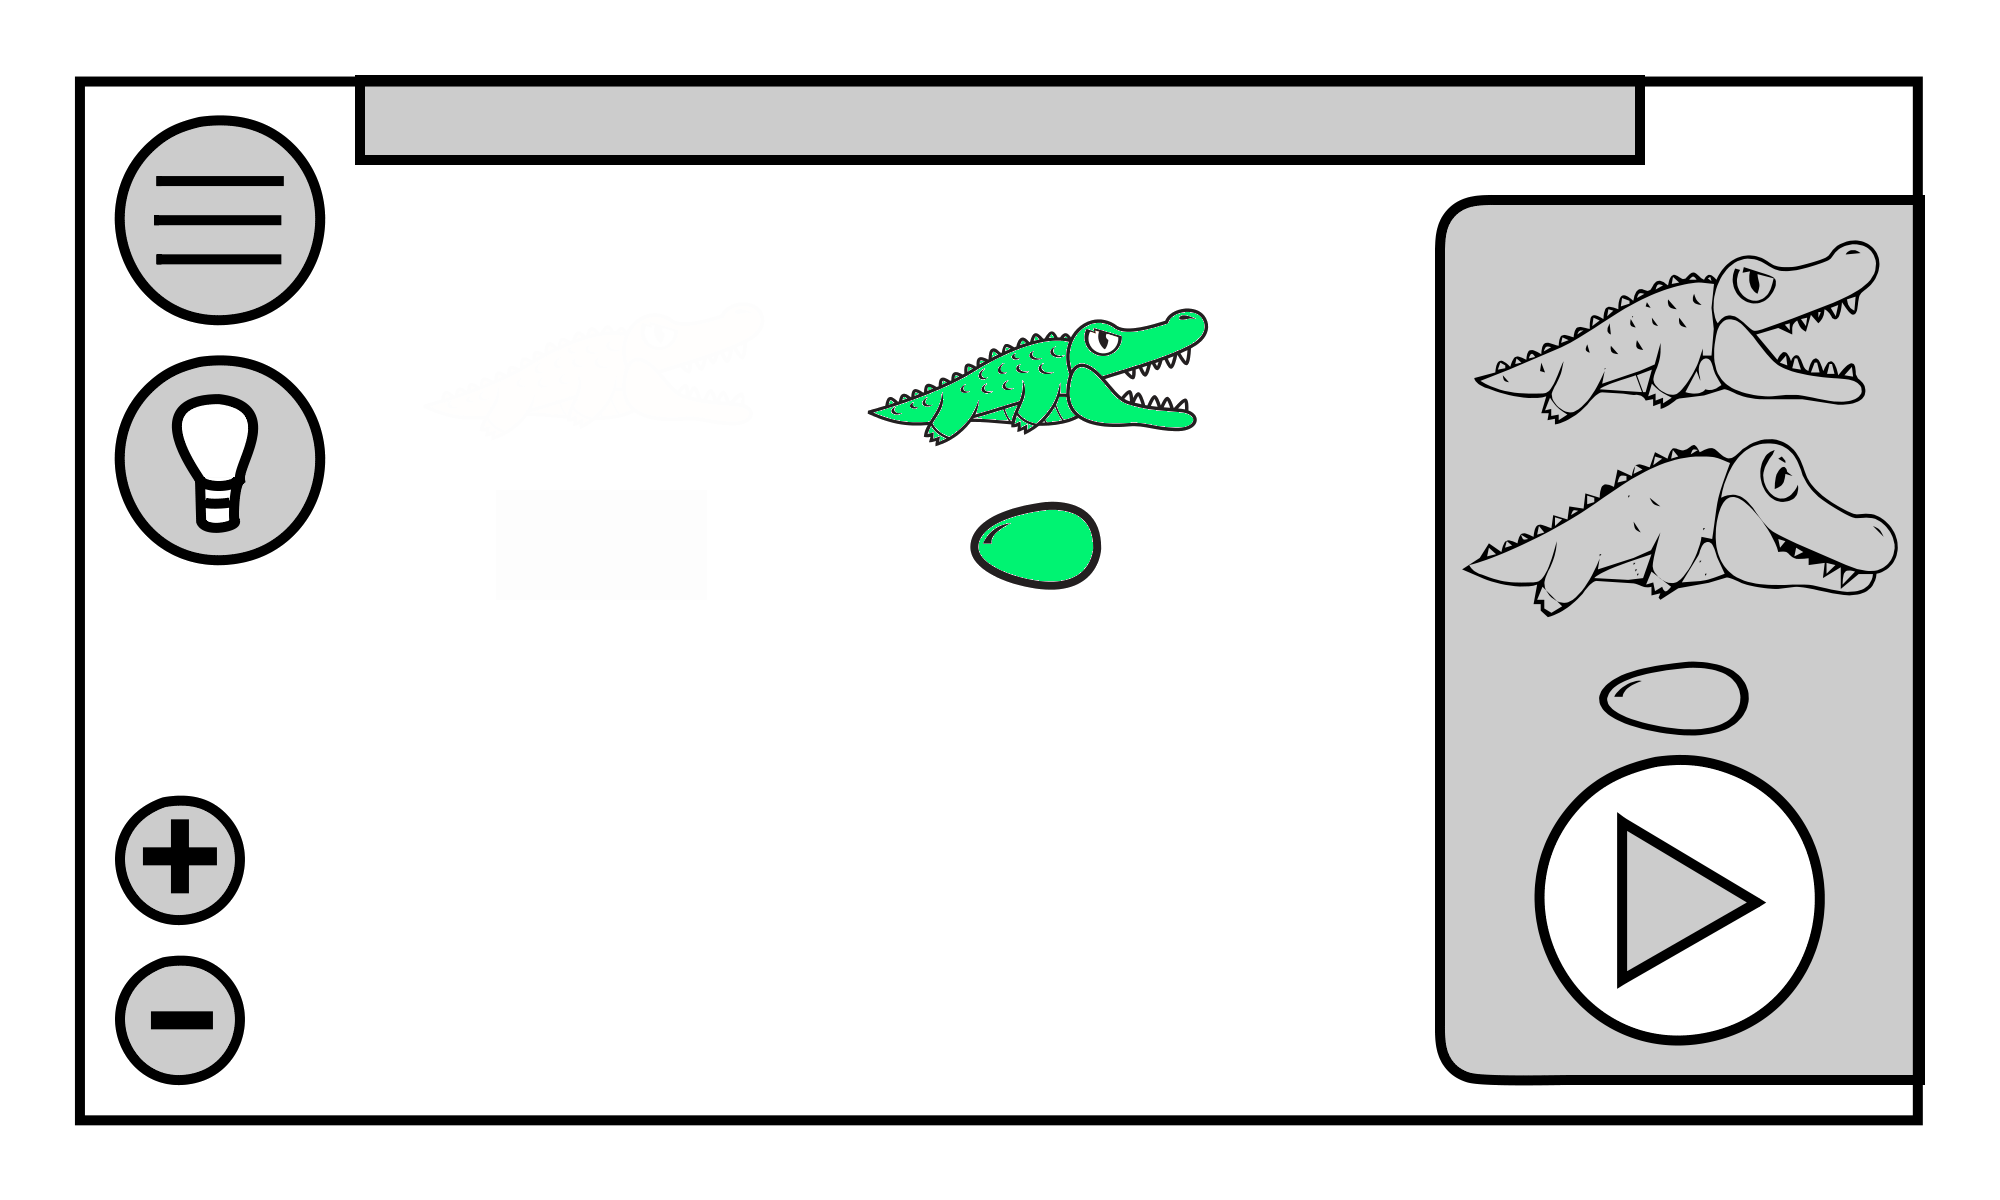
\includegraphics[height=\textheight]{level_end.png}
\end{frame}
\begin{frame}
	\frametitle{Bedienung}
	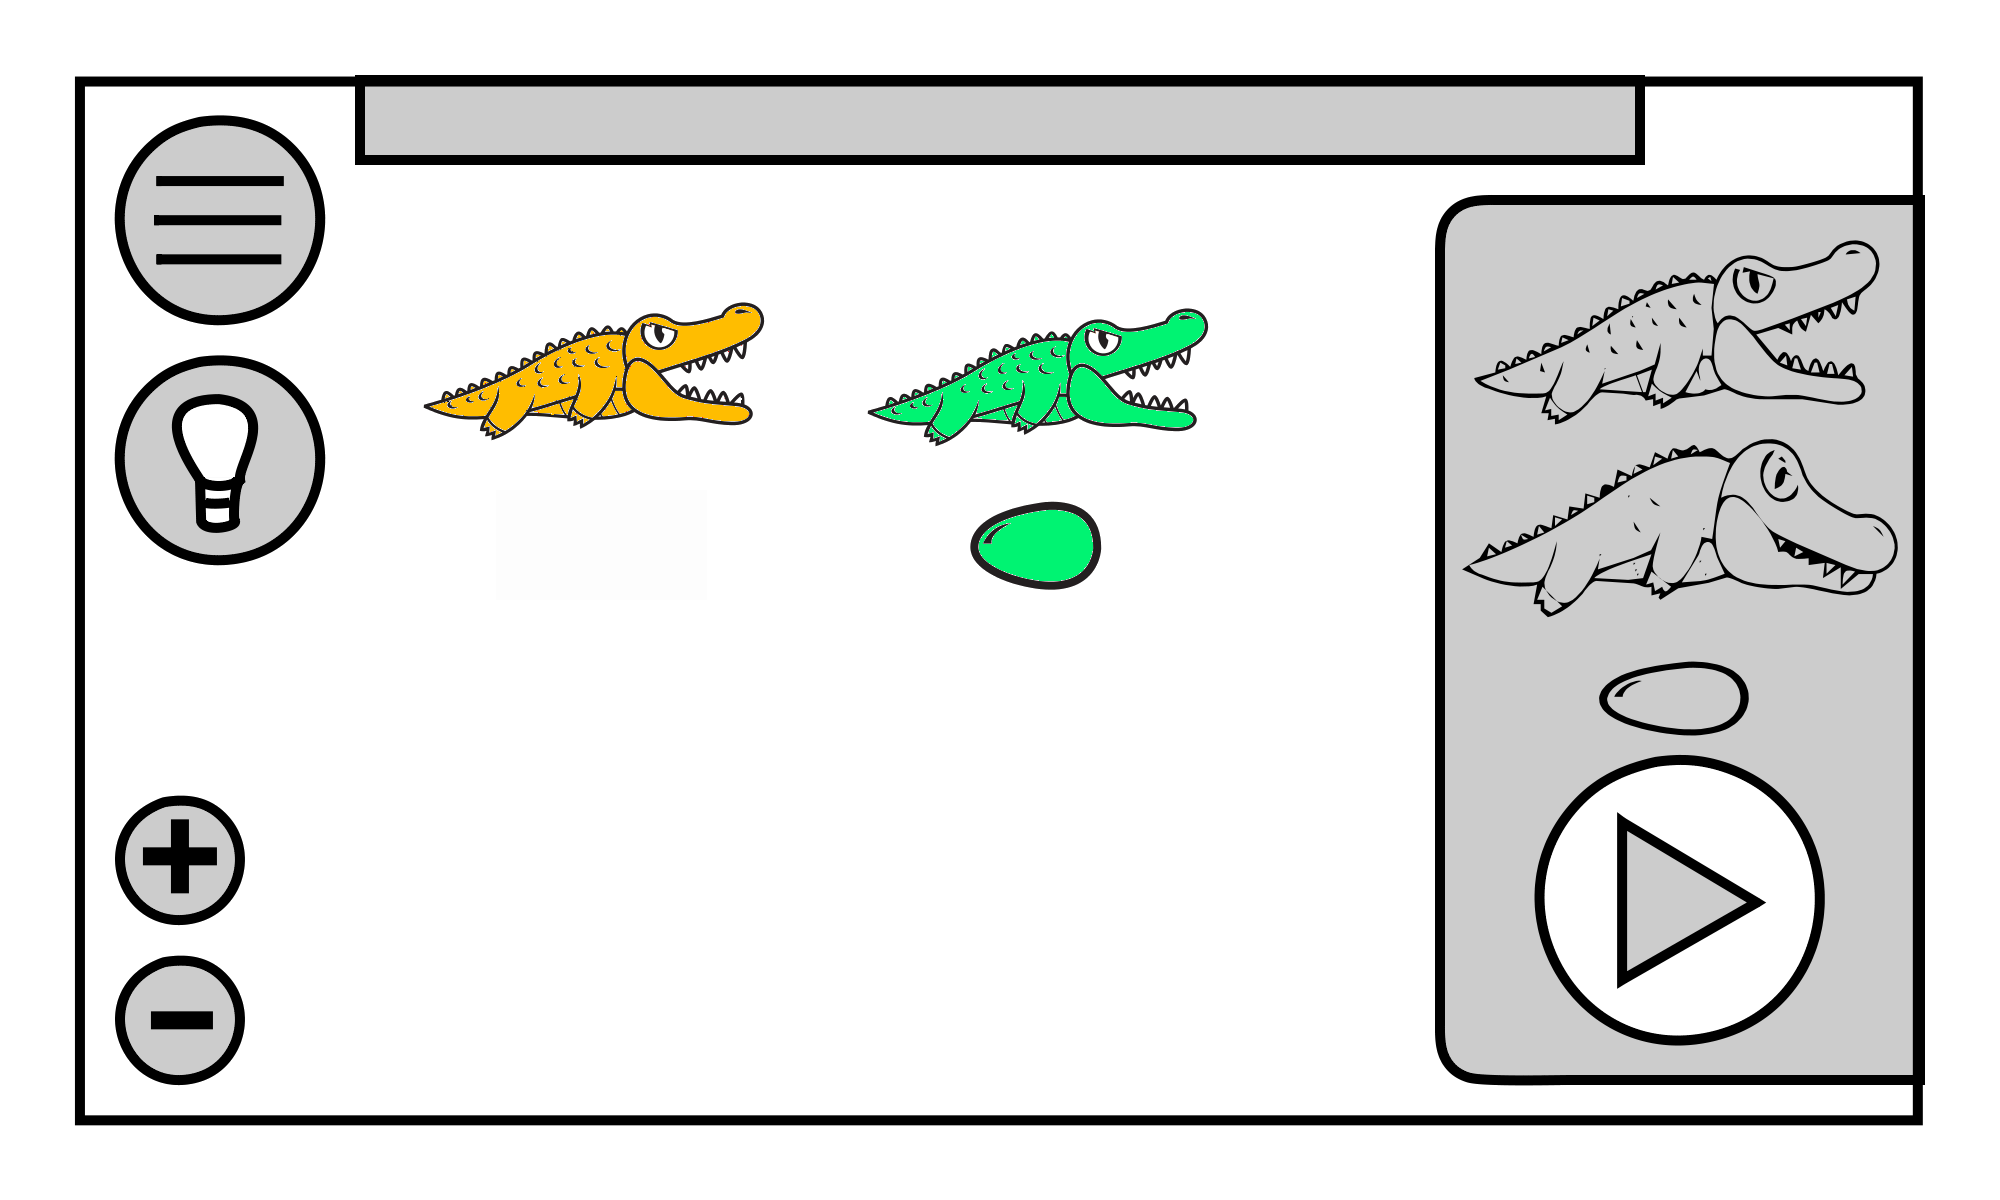
\includegraphics[height=\textheight]{level_start.png}
\end{frame}
\begin{frame}
	\frametitle{Bedienung}
	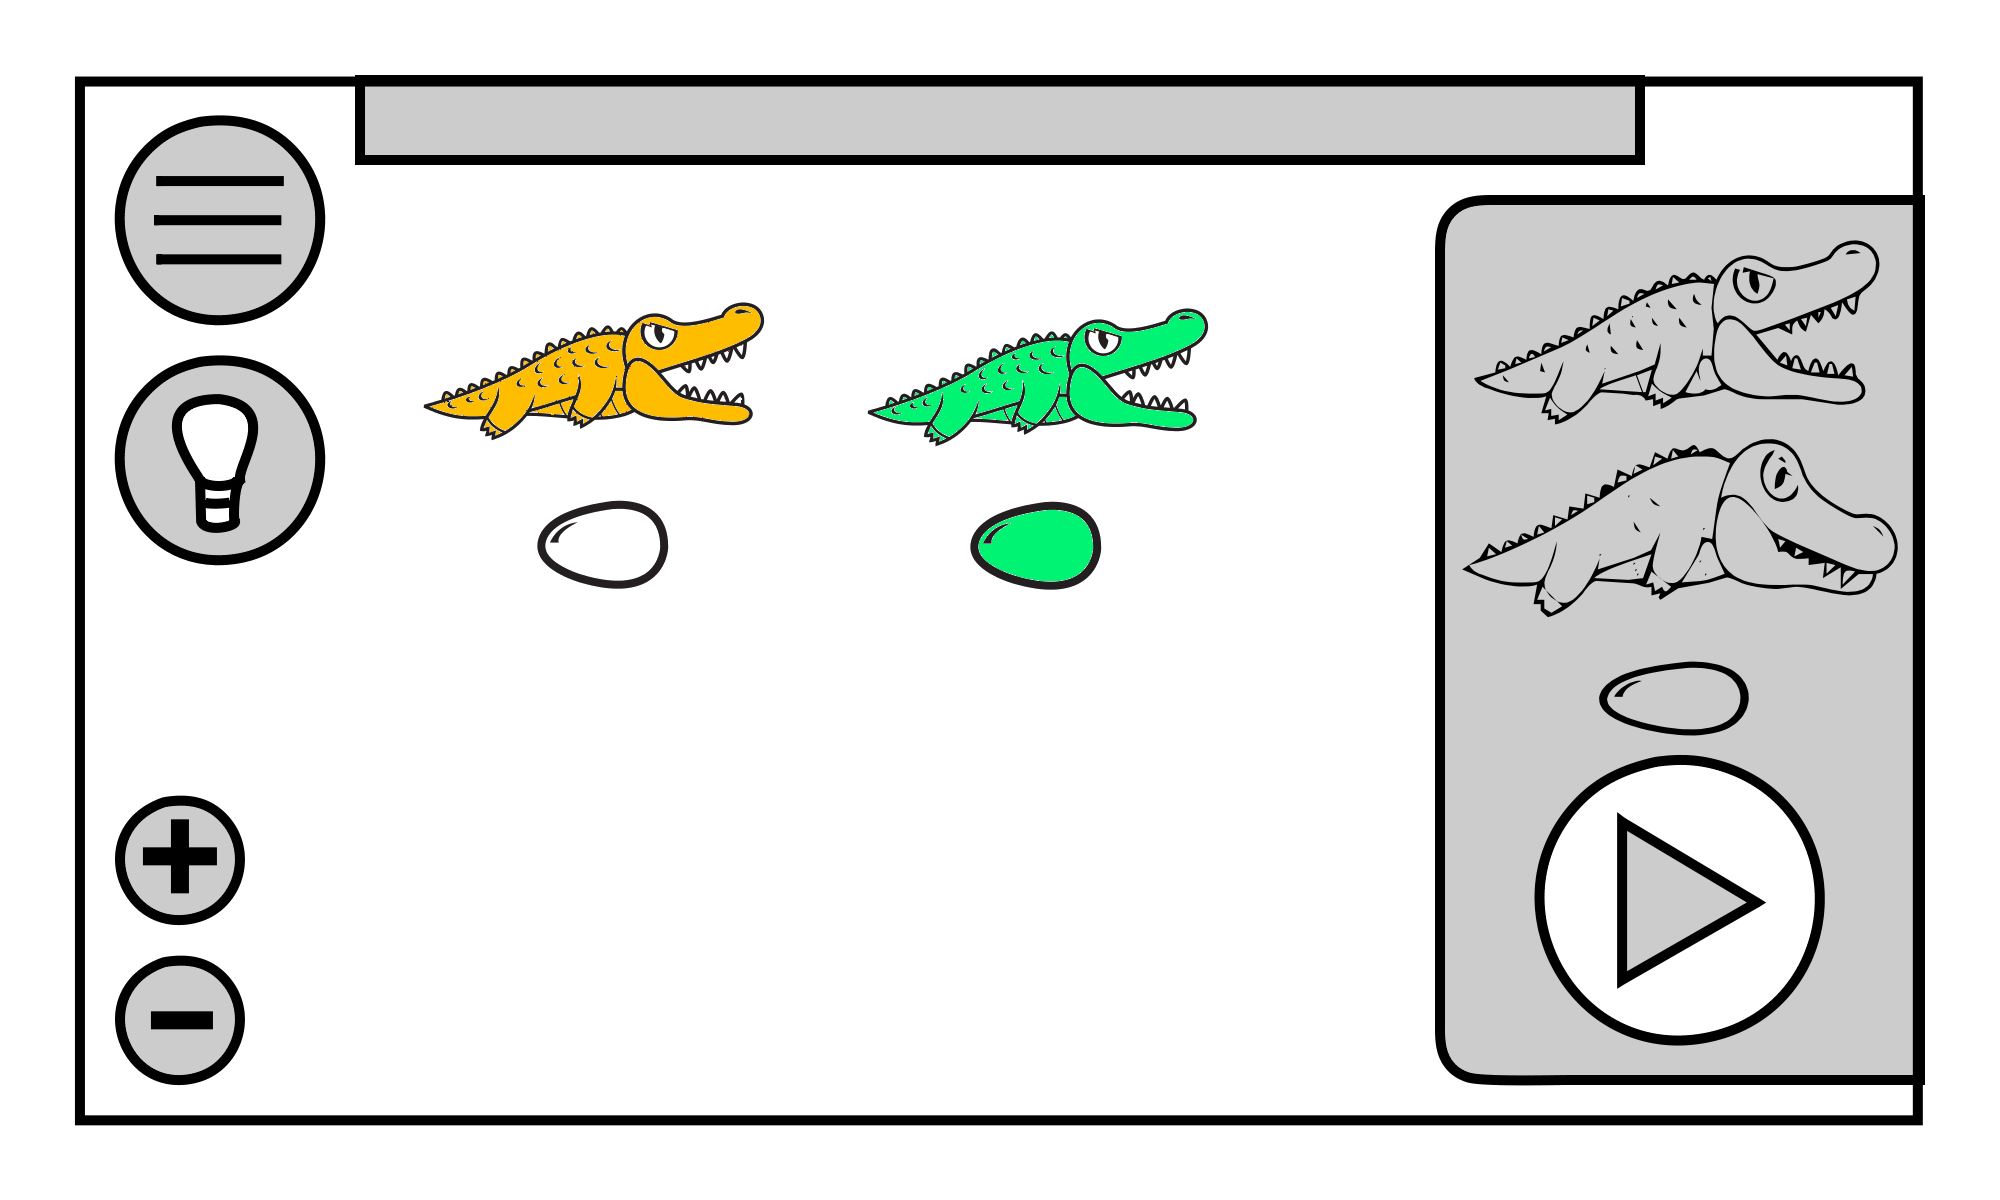
\includegraphics[height=\textheight]{level_colored_croc.png}
\end{frame}
\begin{frame}
	\frametitle{Bedienung}
	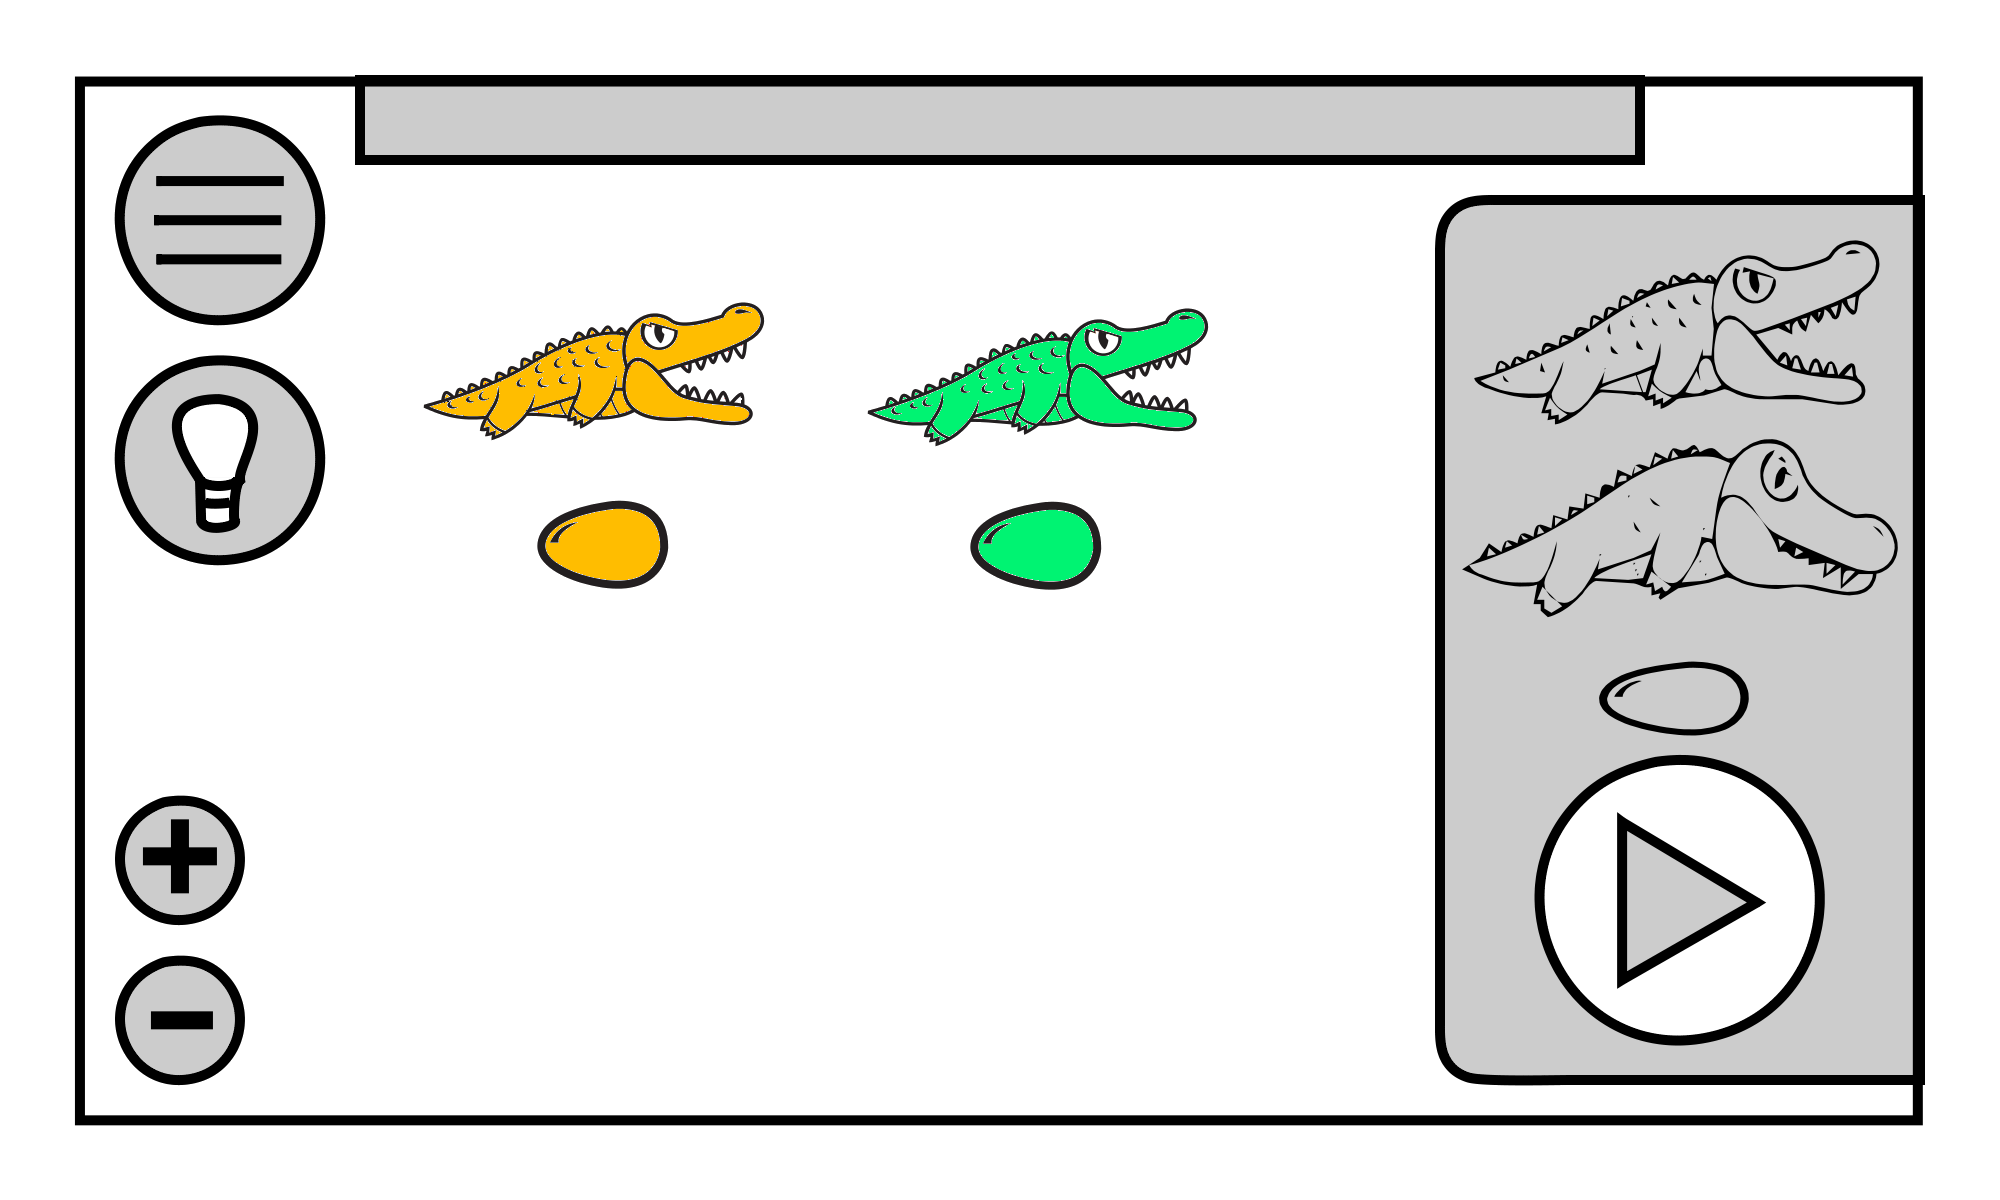
\includegraphics[height=\textheight]{level_colored.png}
\end{frame}
\begin{frame}
	\frametitle{Bedienung}
	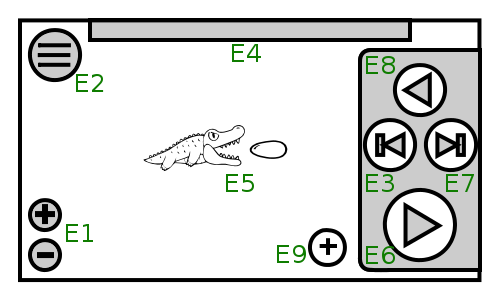
\includegraphics[height=\textheight]{level_simulation.png}
\end{frame}
\begin{frame}
	\frametitle{Motivation}
	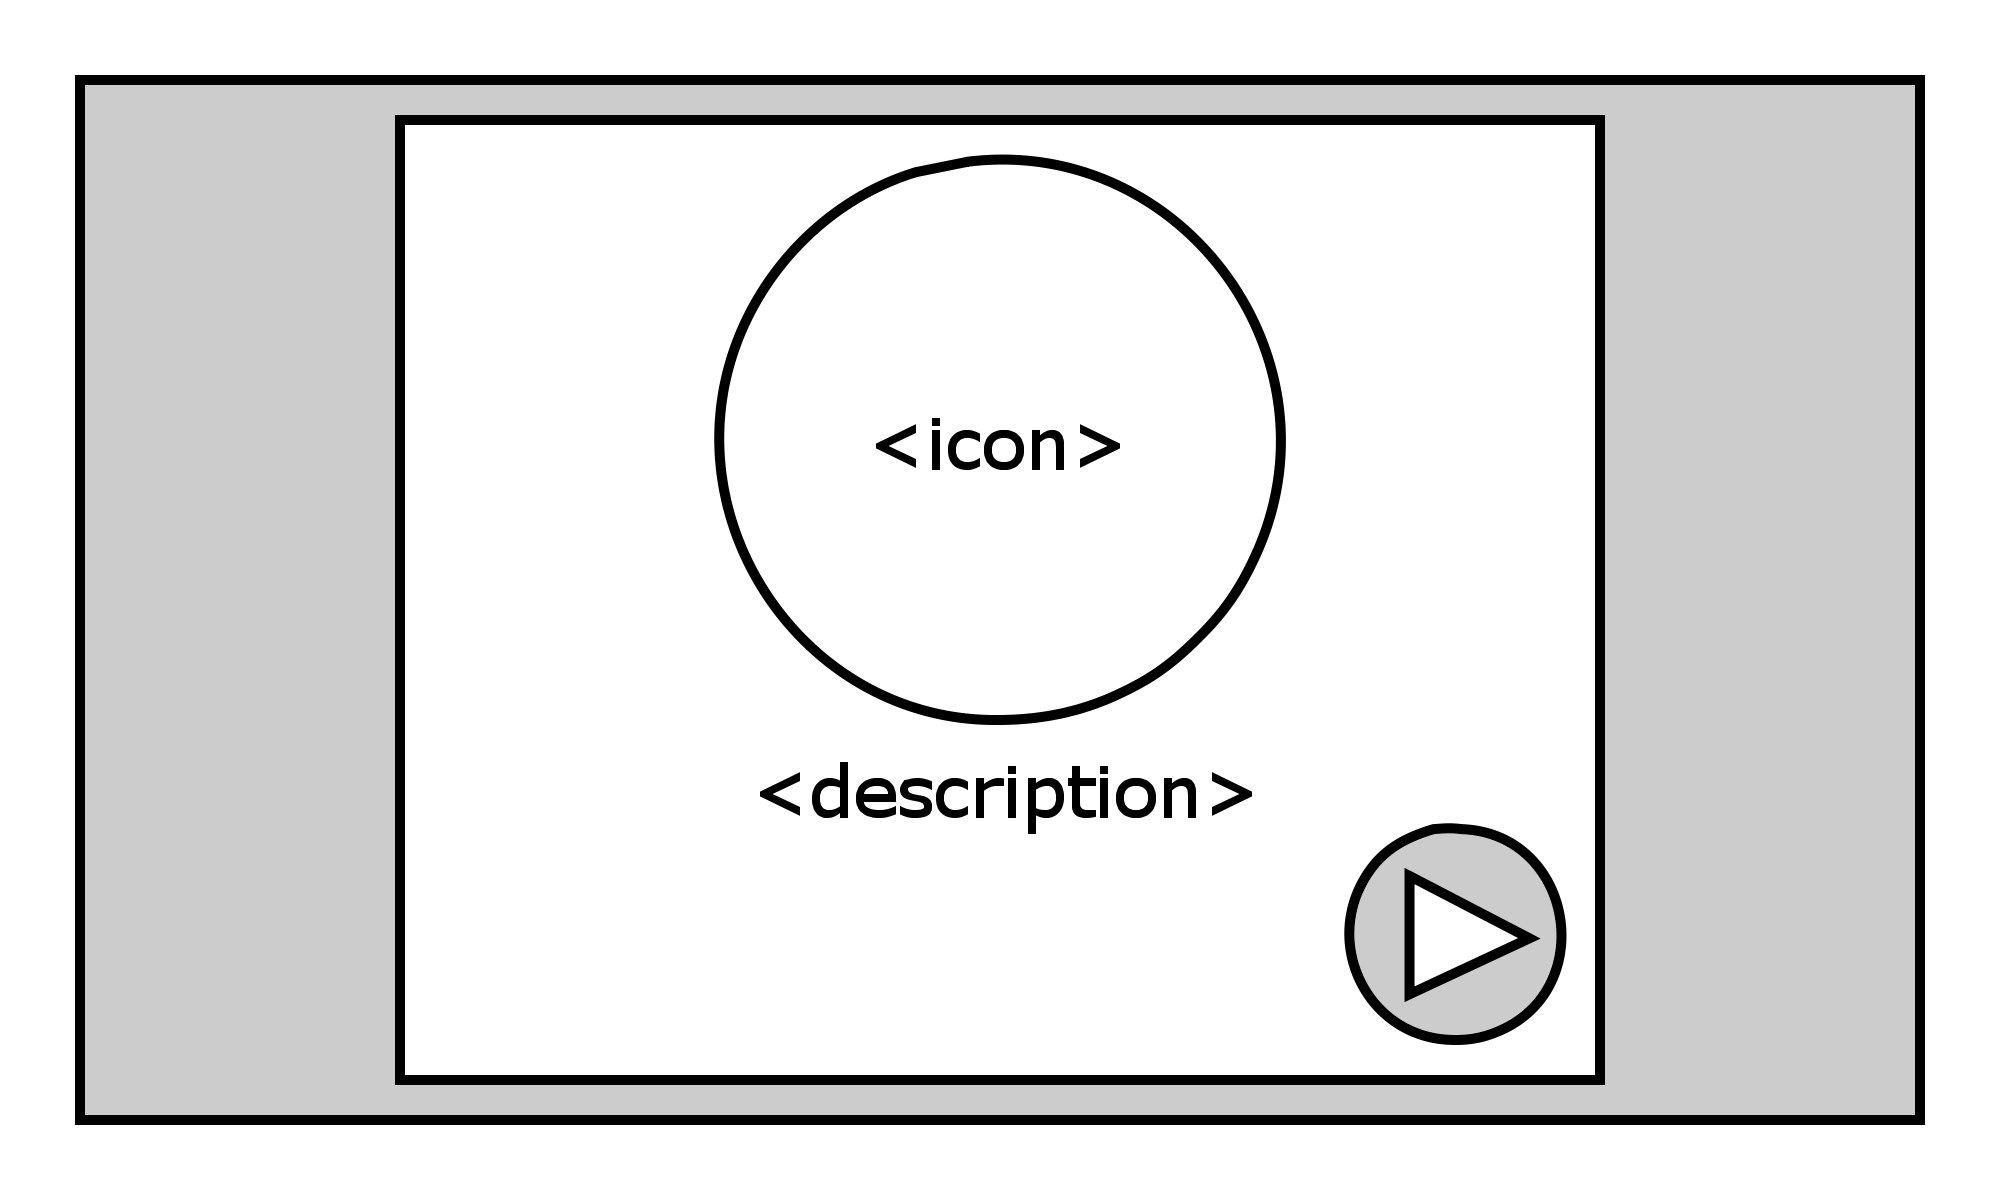
\includegraphics[height=\textheight]{achievement_notification.png}
\end{frame}
\begin{frame}
	\frametitle{Motivation}
	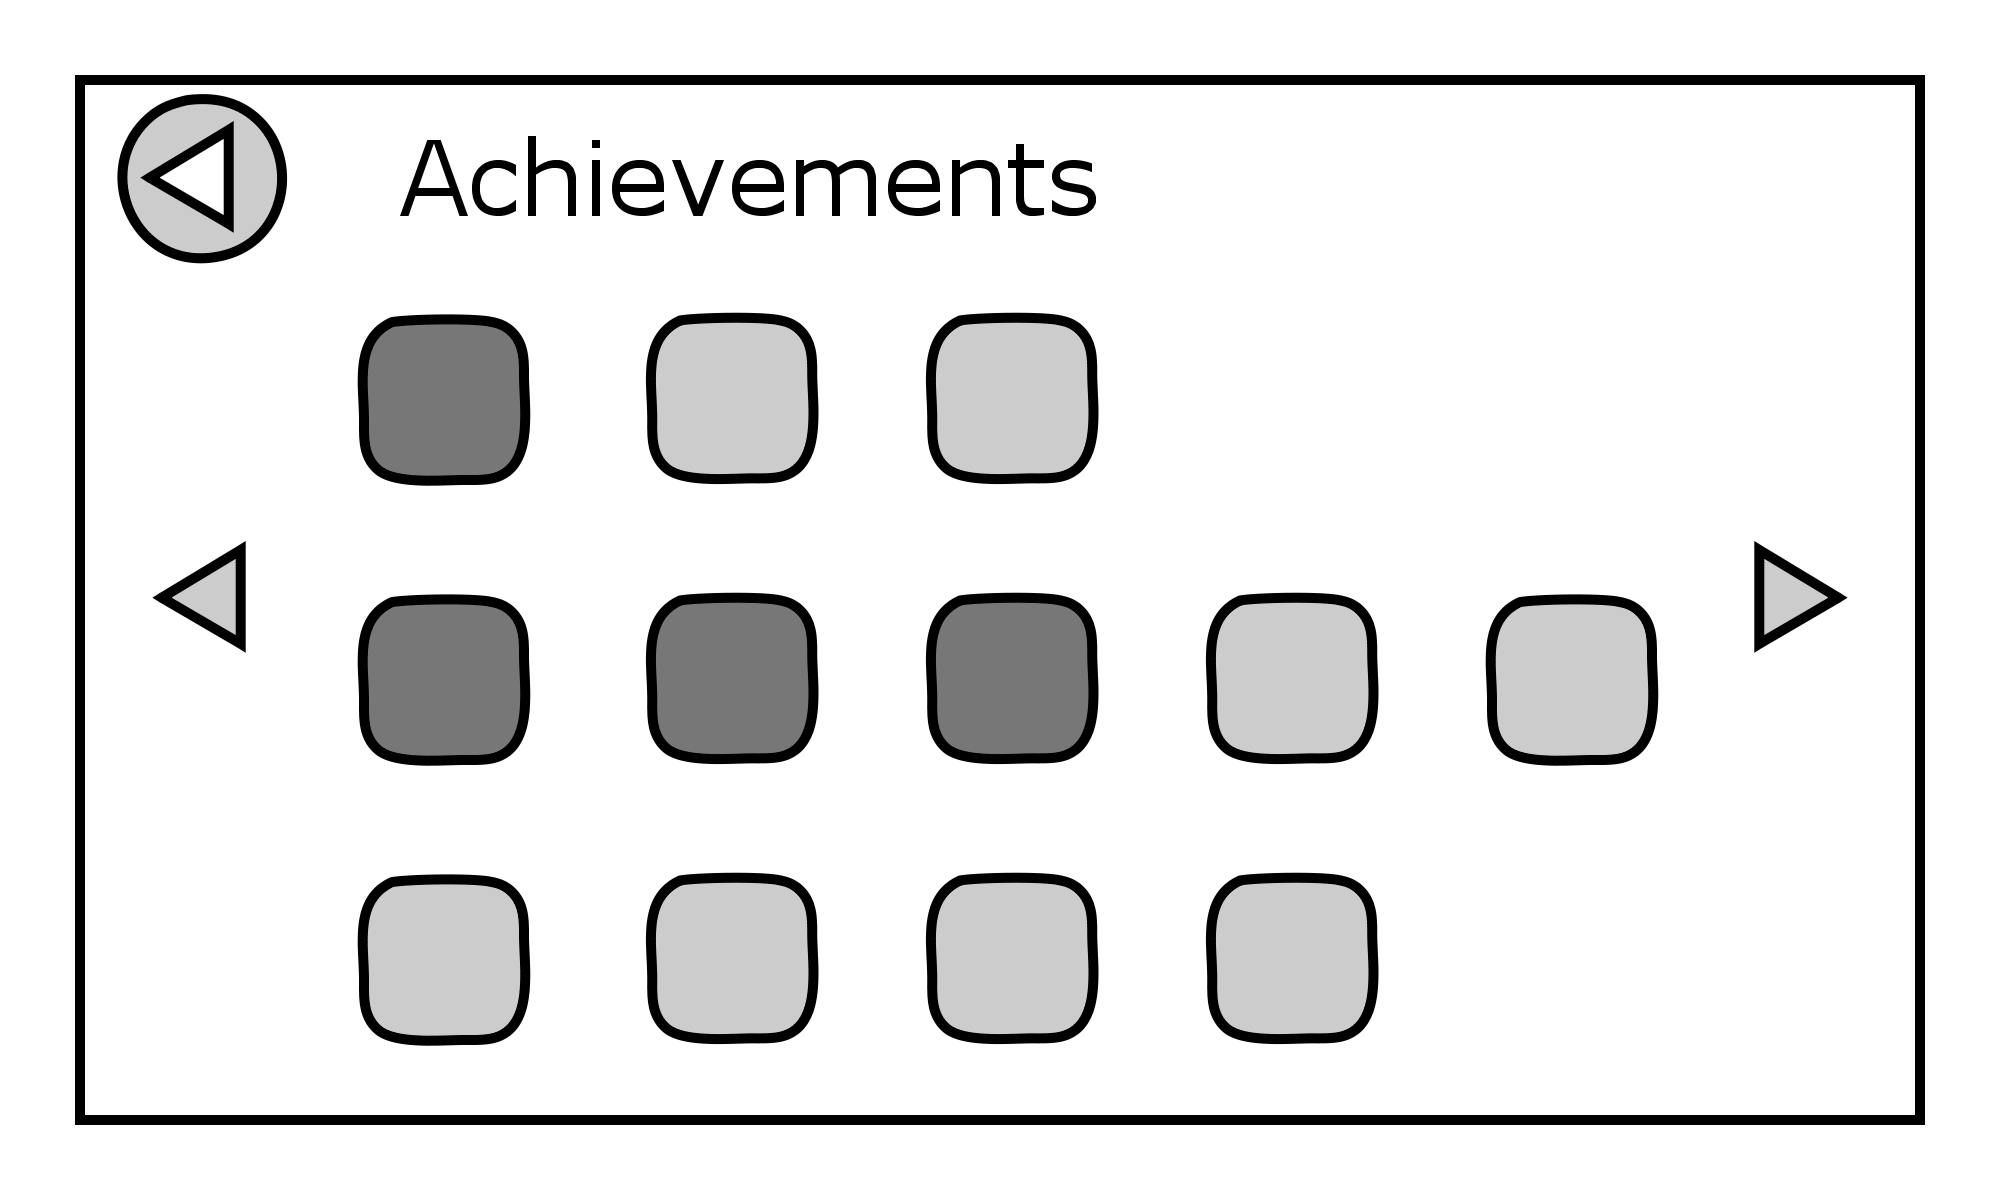
\includegraphics[height=\textheight]{achievements.png}
\end{frame}
\begin{frame}
	\frametitle{Lernkontrolle}
	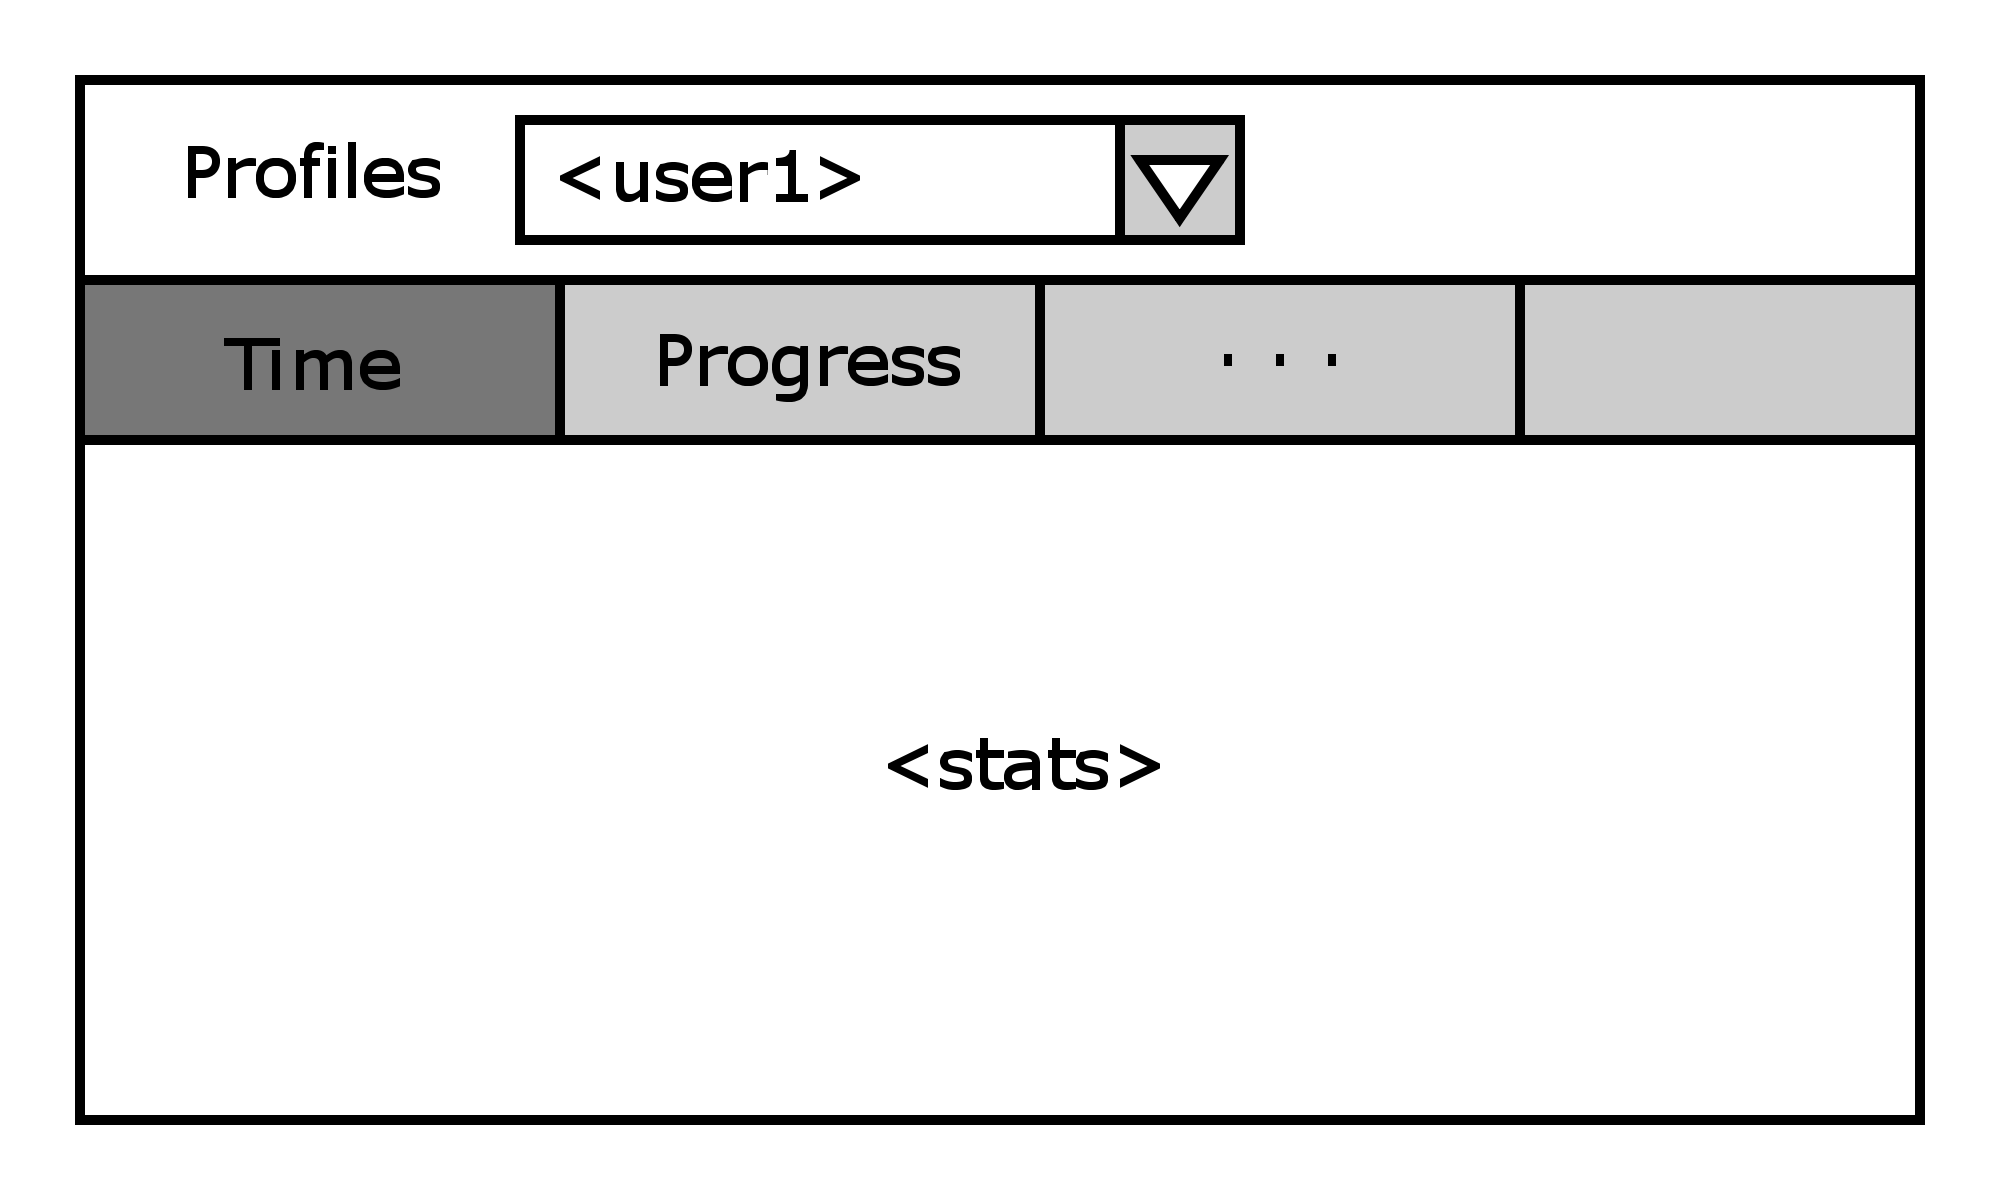
\includegraphics[height=\textheight]{stats.png}
\end{frame}

\end{document}
